\chapter{Experiments and Results}
\label{chap:experiments}

% TODO maybe get rid of this section
\section{Problem Statement}
\label{sec:problem_statement}

In the Deep Q-Network section (\ref{sec:dqn})
I described an approach to deep reinforcement learning.
While the approach works well,
it has not managed to beat all games under consideration
nor would it generalize well to just any game
that fits the input description.
Much care has been taken to make DQN as generic as possible,
yet one detail stands out.

A single state consists of four consecutive image frames
in order to make the problem more Markovian,
a useful trait because it allows us to rely on
useful theoretical properties that have been established
for Markov settings.
However, not all games carry sufficient information
in the last four frames alone.
Some need a few more,
while others could conceivably
show information
that will then be needed to act correctly
after a long period of time has passed.
In other words, there could be hidden state
that the agent nevertheless had access to
at some point in the past.

\paragraph{}
My goal is now to explore different approaches
to this fixed-window history approach,
to explore different ways of dealing with time.
Ideally,
the learning technique should not employ an approach
that contains a fixed window anywhere at all.
However, such techniques are considered here as well.
% TODO discuss POMDP

\paragraph{}
The rest of this chapter is organized as follows.
First, I will examine the Arcade Learning Environment
in close detail in so far as this benefits
the following sections.
Then, I will closely investigate three approaches
to the time problem.
The three techniques discussed in this thesis are
\textit{Late Fusion},
\textit{3D Convolutions}
and \textit{LSTMs}.
Each in turn will be discussed,
then explored and evaluted.
Finally,
I will draw the conclusions of this thesis
in \ref{sec:conclusions}.

\section{Arcade Learning Environment}
\label{sec:arcade_learning_environment}
In order to fully understand the experiments that follow
and the implications of their results,
it is important to first have a closer
look at the Arcade Learning Environment
\parencite{bellemare13arcade}.
ALE is built on top of Stella
\footnote{http://stella.sourceforge.net},
an open-source Atari emulator.
It enables one to programmatically interact
with any compatible Atari game file.
This includes getting the screen in raw pixels,
access to the Atari's emulated RAM,
the game's current score
and actually interacting with the game by sending actions.

\paragraph{}
To appreciate the setting completely we will need to
investigate the hardware the games considered here used to run on.
The Atari 2600 was released in 1977.
Its CPU ran at 1.19 Mhz,
more than a 1000 times slower
than a single average core used for personal computers nowadays.
The size of the RAM was especially small compared to
what is used in modern days, with 128 bytes.

Of special interest to us is the console's graphic component.
The screen is 210 by 160 pixels
and could display up to 128 colors.

The Atari 2600 console is interacted with using
a joystick and a button.
The joystick can move in 8 directions.
Combining that,
along with pushing the button
while moving the joystick
(or not moving it)
gets us to 17 distinguishable actions.
Add one for not doing anything at all
and we have a total of 18 actions for our learning agent.

% TODO consider getting rid of this,
% just thought it was nice to see wtf it is
\begin{figure}[h]
\center
\begin{subfigure}[t]{.5\textwidth}
  \centering
  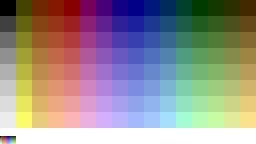
\includegraphics[width=\textwidth]{ntsc_palette.png}
  \vspace{.1\baselineskip}
  \caption{
    The Atari 2600 NTSC Palette used by many games.
    It allows 3 bytes for luminiscence
    and 4 bytes for chrominance,
    resulting in the 128 distinct colors
    you see here.
  }
  \label{fig:nips_network}
\end{subfigure}
\hfill
\begin{subfigure}[t]{.4\textwidth}
  \centering
  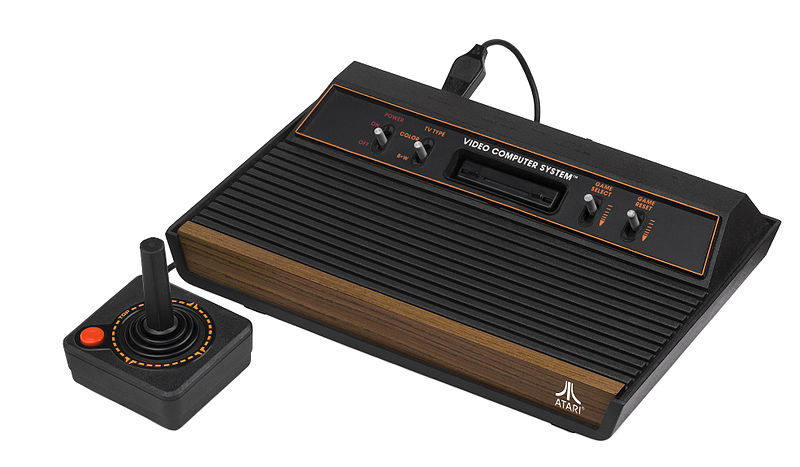
\includegraphics[width=\textwidth]{atari.jpg}
  \vspace{.1\baselineskip}
  \caption{
    The Atari 2600 with its joystick.
  }
  \label{fig:nature_network}
\end{subfigure}
\caption{}
\label{fig:dqn_networks}
\end{figure}

\subsection{Shortcomings}
\label{sub:shortcomings}
While the Atari's computational simplicity,
small screen
and relatively straightforward games
make it a great testbed for reinforcement learning,
the same characteristics
bring along a few shortcomings
that bear discussing.

\paragraph{}
First off, the Atari 2600
is entirely deterministic.
% TODO really want a ref on this
This allows some games to be abused
by learning how to exploit bugs
or otherwise causing situations
that would be very hard for a human to replicate,
yet that a learning algorithm could easily manage
in a deterministic setting.

This exploitation of a game's weak points
does not sound bad on its own
- after all, the agent is learning -
but it is obviously a case of overfitting
which should preferably be avoided.

% TODO should I mention in DQN?
DQN tries to avoid this by adding a random amount
of nullops at the start of the turn,
that is, the agent waits a random amount of turns
before it can play.

\paragraph{}
The console's determinism makes it so
that given the agent's history,
the next state given an action
can be known exactly.
However,
very few games actually need more than
a few frames of history
in order to achieve this Markov property.

Since the main interest of this thesis
is dealing with time,
long-term time dependencies would be especially interesting to investigate.
Sadly, however good of a testing environment ALE may seem,
it lacks thoroughly in this regard.
% TODO erase this if you don't
I will discuss later how to circumvent this lack of complexity partially.

\paragraph{}
% TODO(final) adjust if needed
I will now discuss two games in some detail
and shed light on their core distinctions
in order to later understand and explain
the differences between their learning results.

\subsection{Space Invaders}
\label{sub:space_invaders}
Space Invaders is an arcade game published in 1978.
The player controls a laser cannon
which it can move along the bottom of the screen
and to fire at aliens that move left to right and gradually downwards
and can even shoot back.
The player can even hide below shields
which can get destroyed by lasers from either side.
As the player progresses,
the aliens start to move faster and faster.
The game is over
once they reach the bottom of the screen.

\begin{figure}[htpb]
  \centering
  \begin{subfigure}[t]{.49\textwidth}
    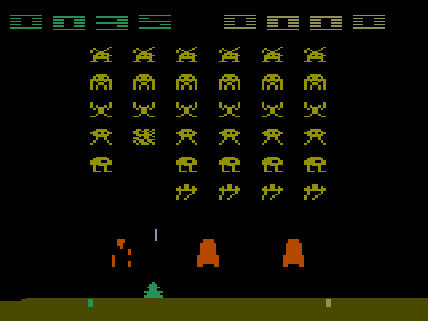
\includegraphics[width=1\textwidth]{space_invaders.png}
  \end{subfigure}
  \begin{subfigure}[t]{.49\textwidth}
    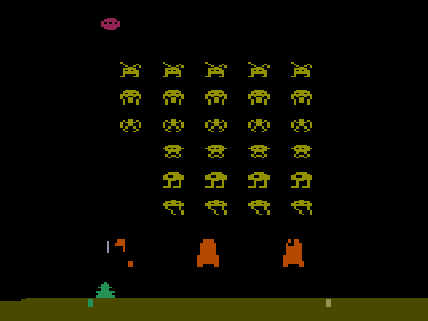
\includegraphics[width=1\textwidth]{space_invaders2.png}
  \end{subfigure}
  \caption{Space Invaders}
  \label{fig:space_invaders}
\end{figure}

Each time an alien gets killed the agent gets a reward
that depends on the type.
The agent needs to learn to associate this reward
with the action that ultimately caused it,
namely firing at the place where an alien would be
at the time the laser arrives.
This can be rather tricky as aliens
can move in multiple directions,
so ideally the agent must somehow learn this pattern
in order to excel at the game.

An agent receives a large bonus reward
when it destroys a periodically appearing fast-flying saucer
at the top of the screen.
This event is especially hard to learn because
of its rarity compared to other situations.


\subsection{Pong}
\label{sub:pong}
Pong was originally an arcade game by Atari.
It was then ported to the Atari 2600
under the name \textit{Video Olympics},
% TODO uuuh
though in this text I will refer to it simply as Pong.

\begin{figure}[htpb]
  \centering
  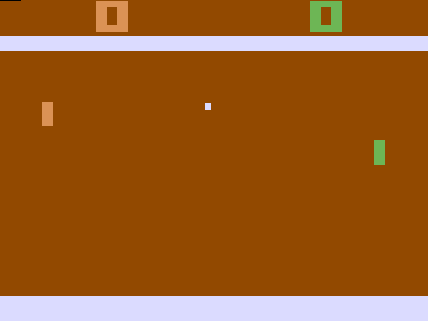
\includegraphics[width=0.5\linewidth]{pong.png}
  \caption{Pong}
  \label{fig:pong}
\end{figure}

The game is a simulation of badmin.
It features two paddles,
each controlled by a different player (or AI).
A ball is hit back and forth between the players
by moving the paddle up and down
% TODO peter 18 frames
and intercepting the ball to bounce it back.
A point is scored when the opponent
fails to do so.

\subsubsection{Flickering Pong}
Since regular Pong and indeed most Atari games
become at least approximately Markovian
given a small history,
we would like a different benchmark
to compare techniques
for partially observable MDP's.
Such a one has been introduced by \citeauthor{Hausknecht2015} (\citeyear{Hausknecht2015})
with \textit{Flickering Pong}.
It is entirely the same game as Pong,
except a frame can only be observed with some probability $p$
and becomes obscured, that is, entirely black, otherwise.
This results in a stochastic screen flickering for the learning agent.

In order to be successful at Flickering Pong,
an agent must learn to robustly
estimate variables such as ball velocity
across multiple frames,
half of which are expected to be obscured.

\paragraph{}
% TODO note on how hausknecht's results were

\section{Stacked Frames Approach}
\label{sec:stacked_frames_approach}
In order to get a better feeling
of why the dimension of time in reinforcement learning
merits closer examination and further research,
this section will elaborate on the current approach
as described by
\citeauthor{Mnih2013} (\citeyear{Mnih2013}).
\citeauthor{Mnih2013}
found that for most games under discussion
4 frames of history is sufficient to render the game approximately Markovian.
This means that when considering not only a single frame
but also the 3 prior to it,
all information that could ever be required to make an optimal decision
at that point is encompassed within this small fixed window.

\paragraph{}
In order to combine these frames,
it is sufficient to make sure each image frame only has a single image channel
(e.g. grayscale or luminiscence)
so the image depth dimension can be reused
to simply stack the frames on top of each other.
This limitation is present because 2D convolutional networks
can only handle three dimensions,
of which over the third one has no control in terms of filter size;
it always reaches across the whole depth.

This way of stacking frames along with the rest of the standard DQN
is depicted in Figure \ref{fig:nips_network2}.

\begin{figure}[htpb]
  \centering
  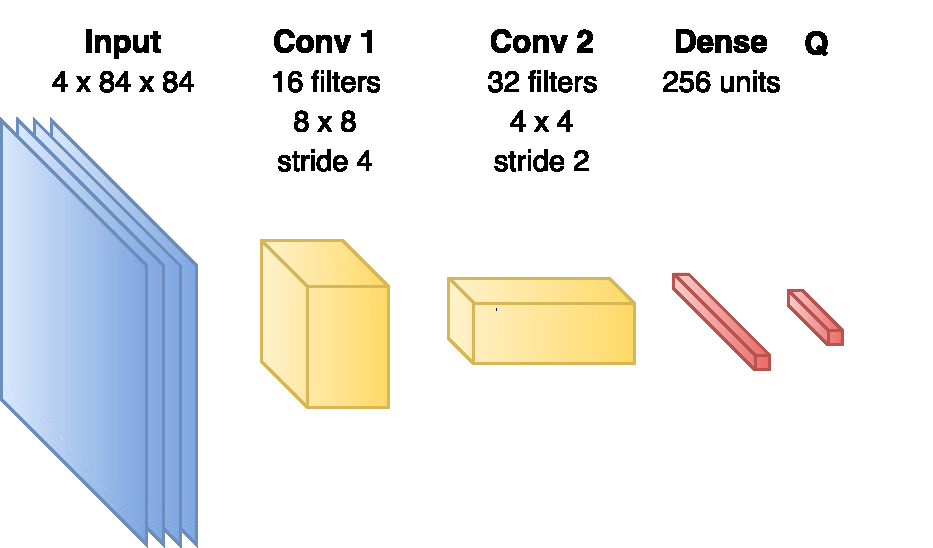
\includegraphics[width=0.8\linewidth]{nips_network2.pdf}
  \caption{DQN architecture by \cite{Mnih2013}.
    Note that the frames can not have any depth because of
    the limitations imposed by 2D convolutions.
  }
  \label{fig:nips_network2}
\end{figure}

In order to determine
whether this frame stacking approach
actually benefited from the extra history,
I investigated multiple
the learning process for multiple games
with both architectures.
We are interested in the learning curve
which can be characterized with
total accumulated reward over time,
as suggested by \citeauthor{Bellemare2015} \citeyear{Bellemare2015}.
This is done by periodically
holding greedy playthroughs for 50000 steps
and then averaging the accumulated rewards
over the episodes.

In Figure \ref{fig:stacked_vs_single_rewards}
we can see rewards over time as the agent progresses.
While it does show general tendencies quite well,
the graphs are noisy even though results are averaged over 5 runs.
This is especially the case for DQN with 4 frames.
As \citeauthor{Mnih2013} (\citeyear{Mnih2013}) notes,
this is due to the fact that small policy weight changes
can result in vastly different visited states for the policy.



% TODO peter leuke note: DQN 1 is veeeel steadier in reward :)
\begin{figure}[htpb]
  \centering
  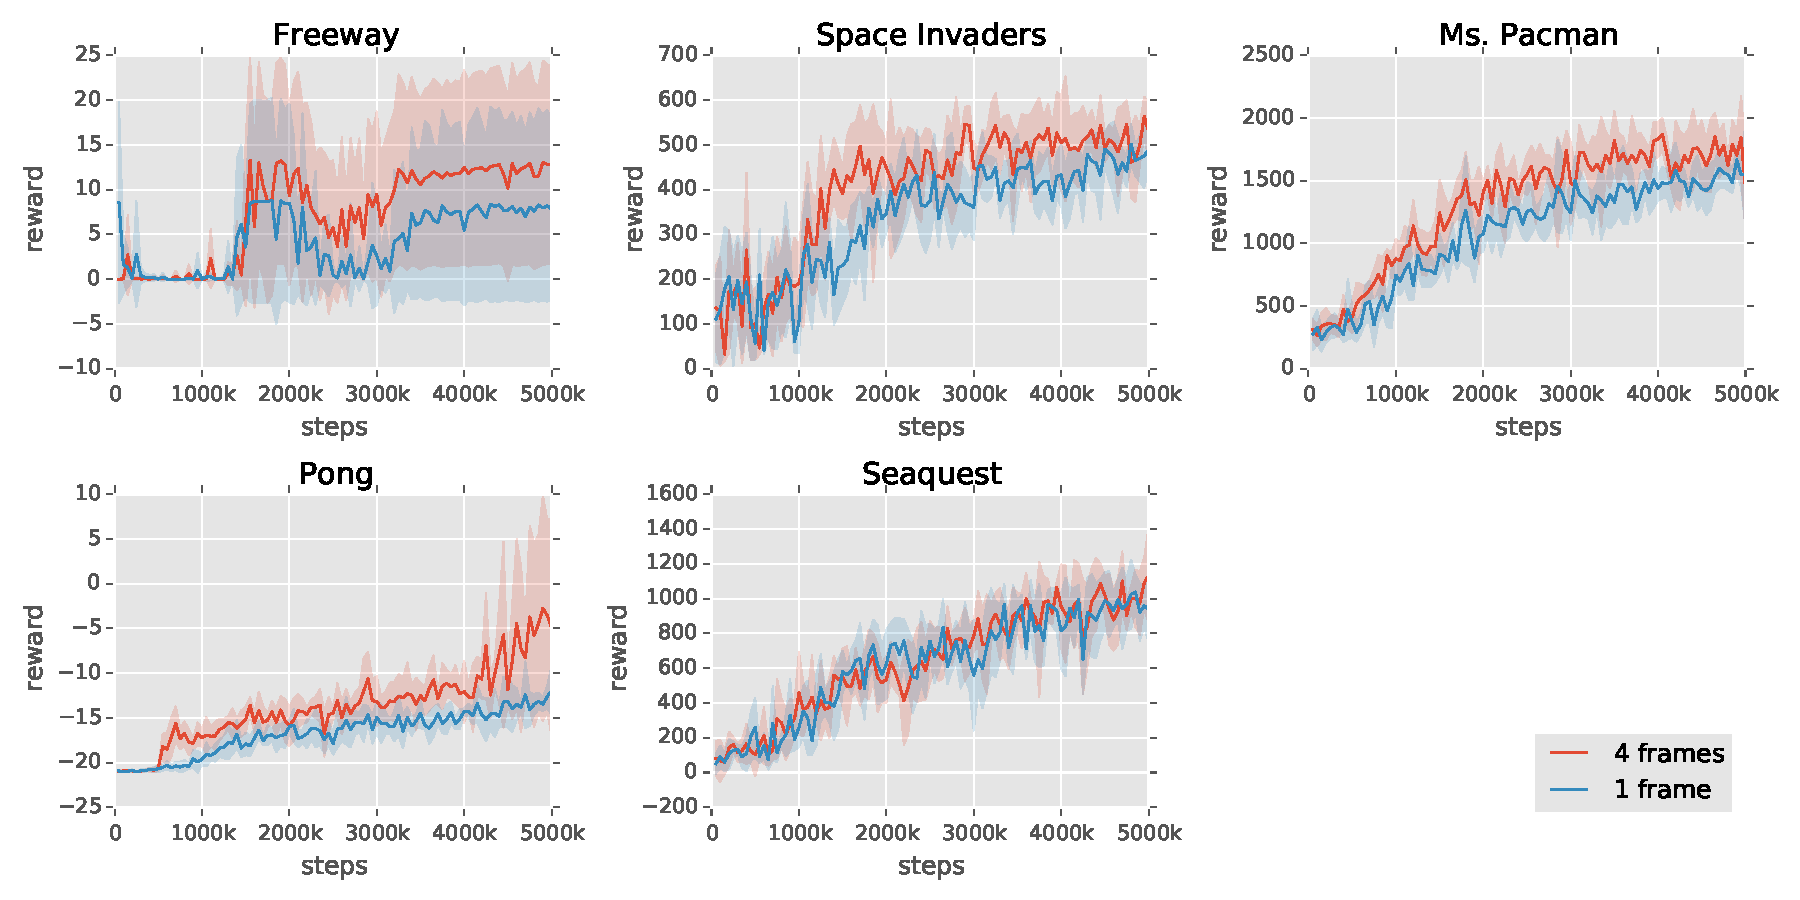
\includegraphics[width=\linewidth]{stacked_vs_single.pdf}
  \caption{
    Rewards over time for 4 stacked frames as input
    compared to just a single one
    for five different games
    with experiment parameters as in Table \ref{tab:boost}.
    % Rewards are smoothed with a weighted running average
    % with a window of 5 frames.
    Shaded areas depict standard error.
  }
  \label{fig:stacked_vs_single_rewards}
\end{figure}

\paragraph{}
It can be often hard to tell if the agent is making steady progress
using the reward curves
and it can be even harder to compare different approaches.
To combat this I will often employ an alternative method
for evaluating an agent's learning behavior.
At the start of a learning experiment, 3200 states are gathered
using a random policy.
Periodically,
for each of these states the maximum Q-value is computed
and the average over all these states then collected
as an indication of learning behavior.

\begin{figure}[htpb]
  \centering
  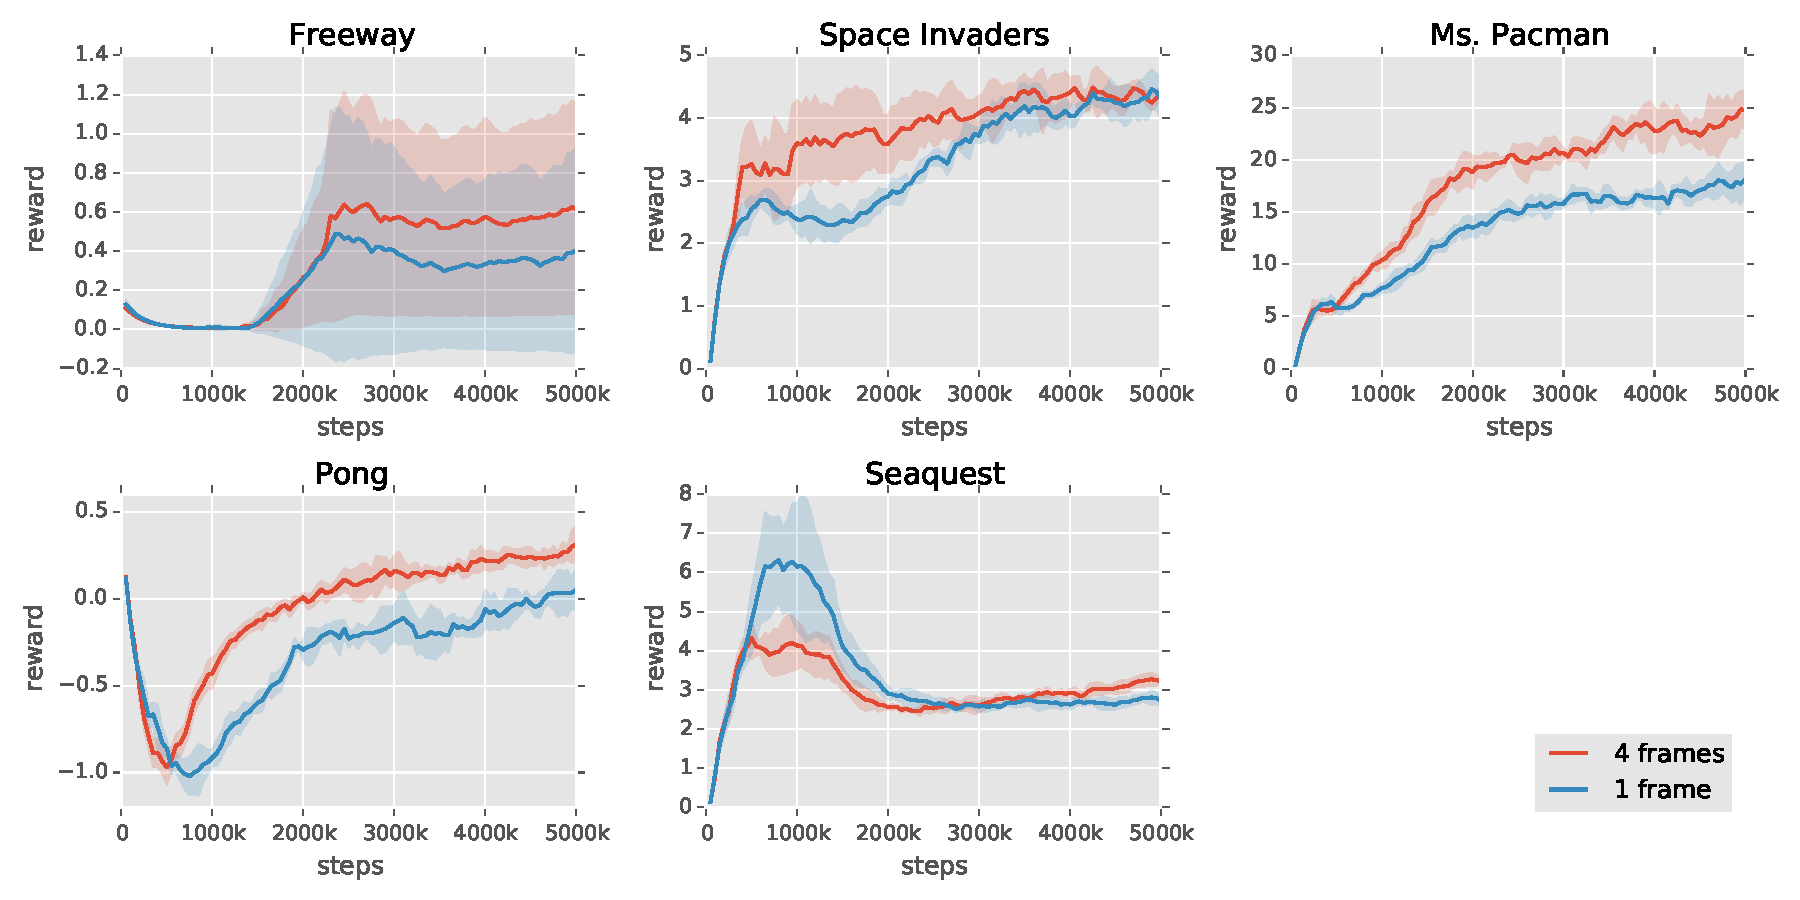
\includegraphics[width=\linewidth]{stacked_vs_single_qs.pdf}
  \caption{
    Average maximum Q-value over time for 3200 holdout states.
    Shaded areas depict standard error.
  }
  \label{fig:stacked_vs_single_qs}
\end{figure}

\paragraph{}
The resulting graphs in Figure \ref{fig:stacked_vs_single_qs}
are much less noisy
and give a decent indication of how well the
different agents learn the games' value functions.
We can now analyse the experiment's results.
For 4 out 5 games we can say that the stacked frames approach
performs noticeably better,
although for the game Freeway results are so noisy
we can not make a strong statement.
The game Seaquest seems to form an outlier
in that the stacked approach forms no immediately obvious advantage.
It does look like it might not have stagnated entirely
and is actually improving beyond the single frame DQN
but we do not have data beyond that point
and it has not helped within the employed 5 million training steps.

\paragraph{}
% TODO peter please mag ik dit zeggen
From this data we can deduce that the stacked approach does
fare better compared to just using a single frame
although it is heavily dependent on each game's specific mechanics.
% TODO peter dit klopt he
What we can not conclude with certainty however
is whether the results are due to the historic information
or increased capacity of the first convolutional layer
in order to cope with the extra frames.


\section{Late Fusion Network Approach}
\label{sec:late_fusion_network_approach}
The first alternative to the standard DQN
considered here is
the Late Fusion DQN architecture
inspired by \citeauthor{Karpathy2014} (\citeyear{Karpathy2014})
who successfully deployed it for
action recognition in video clips.
The base premise for this architecture
is that in order to capture time dependencies
it is sufficient to look at differences
between frames.
Presumably,
this works better with short-term dependencies
as differences between frames close to each other in time
are smaller.

Also, Late Fusion
considers two frames with a fixed distance in time in between.
This can only yield good results for longer time dependencies
if the dependency always spans approximately the same amount of time,
a requirement that is undesirable
and not always satisfiable.

\paragraph{}
The Late Fusion DQN is based on the default DQN implementation.
In fact, the learning algorithm is entirely the same
and parameters are as depicted in Table \ref{tab:base}.

Instead of a single stack of convolutional layers,
we now have two towers that each take as input a single frame.
The frames are separated by a fixed amount of frames
that go unused for the pass.
Each of the two towers has no access to the frame
that is input to the other one.
Rather, the towers get combined by a fully connected layer
that is also the first of the layers that has access
to both time steps.

Since each convolutional network now only has a single frame as input,
we suddenly get back the image channel input dimension (depth)
that was previously used to stack frames together.
In order to use that dimension for time,
DQN uses a grayscale
which only requires a single scalar value
and as such this channel dimension was implicit before.
Now that we have access to an extra input dimension
we can again use color channels
such as RGB,
which might add useful information to the model.

\paragraph{}
The general gist to the Late Fusion architecture
is that the convolutional layers
compute high-level features
which the fully-connected layer can then compare
in order to compute the correct output.

The full architecture is depicted in Figure \ref{fig:late_fusion}.

\begin{figure}[htpb]
  \centering
  % \captionof{figure}{Late Fusion Network}
  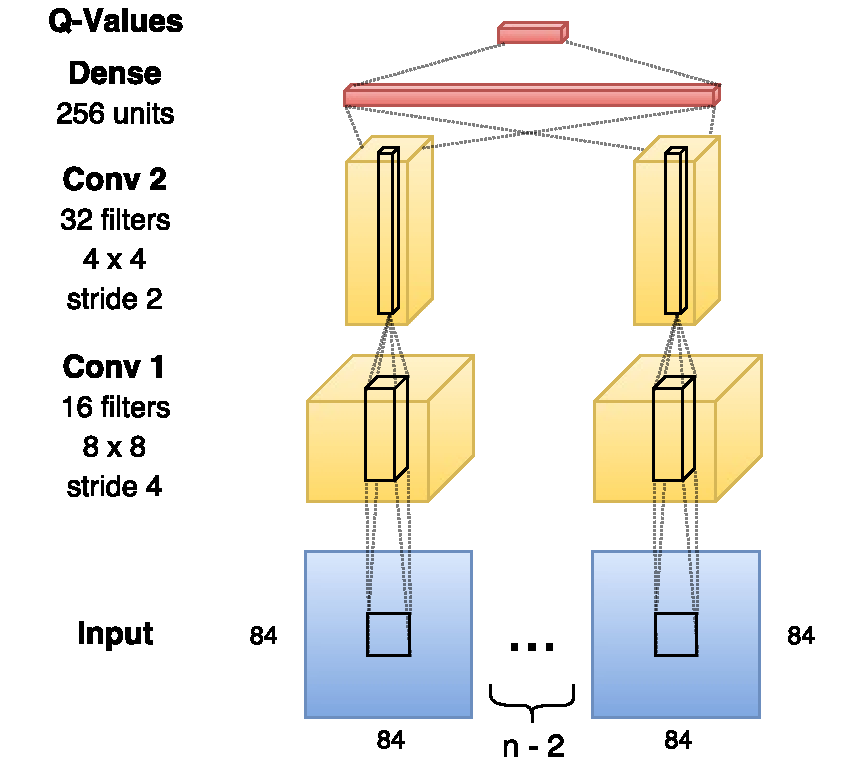
\includegraphics[width=0.8\linewidth]{late_fusion.pdf}
  \caption{
    Late Fusion DQN.
    A sample of $n$ consecutive frames is chosen
    but only the outer two frames
    feed into the network.
    The features learned by the two convolutional networks
    is combined through the fully-connected layer
    that combines both.
    Only from the fully-connected layer up
    is information from two different time steps available.
  }
  \label{fig:late_fusion}
\end{figure}

\subsection{Tuning}
\label{sub:late_fusion_tuning}
We can try a few different alterations to the basic late fusion architecture.
First off we can decide whether convolutional layer weights should be shared
between layers at the same level
or separate for each tower.
Then there is the extra image dimension we have access to.
In order to make use of it,
I used frames with 3 color channels
to hold RGB values.

A performance comparison for the game Pong is depicted in
Figure \ref{fig:late_fusion_pong_rewards}.

\begin{figure}[htpb]
  \centering
  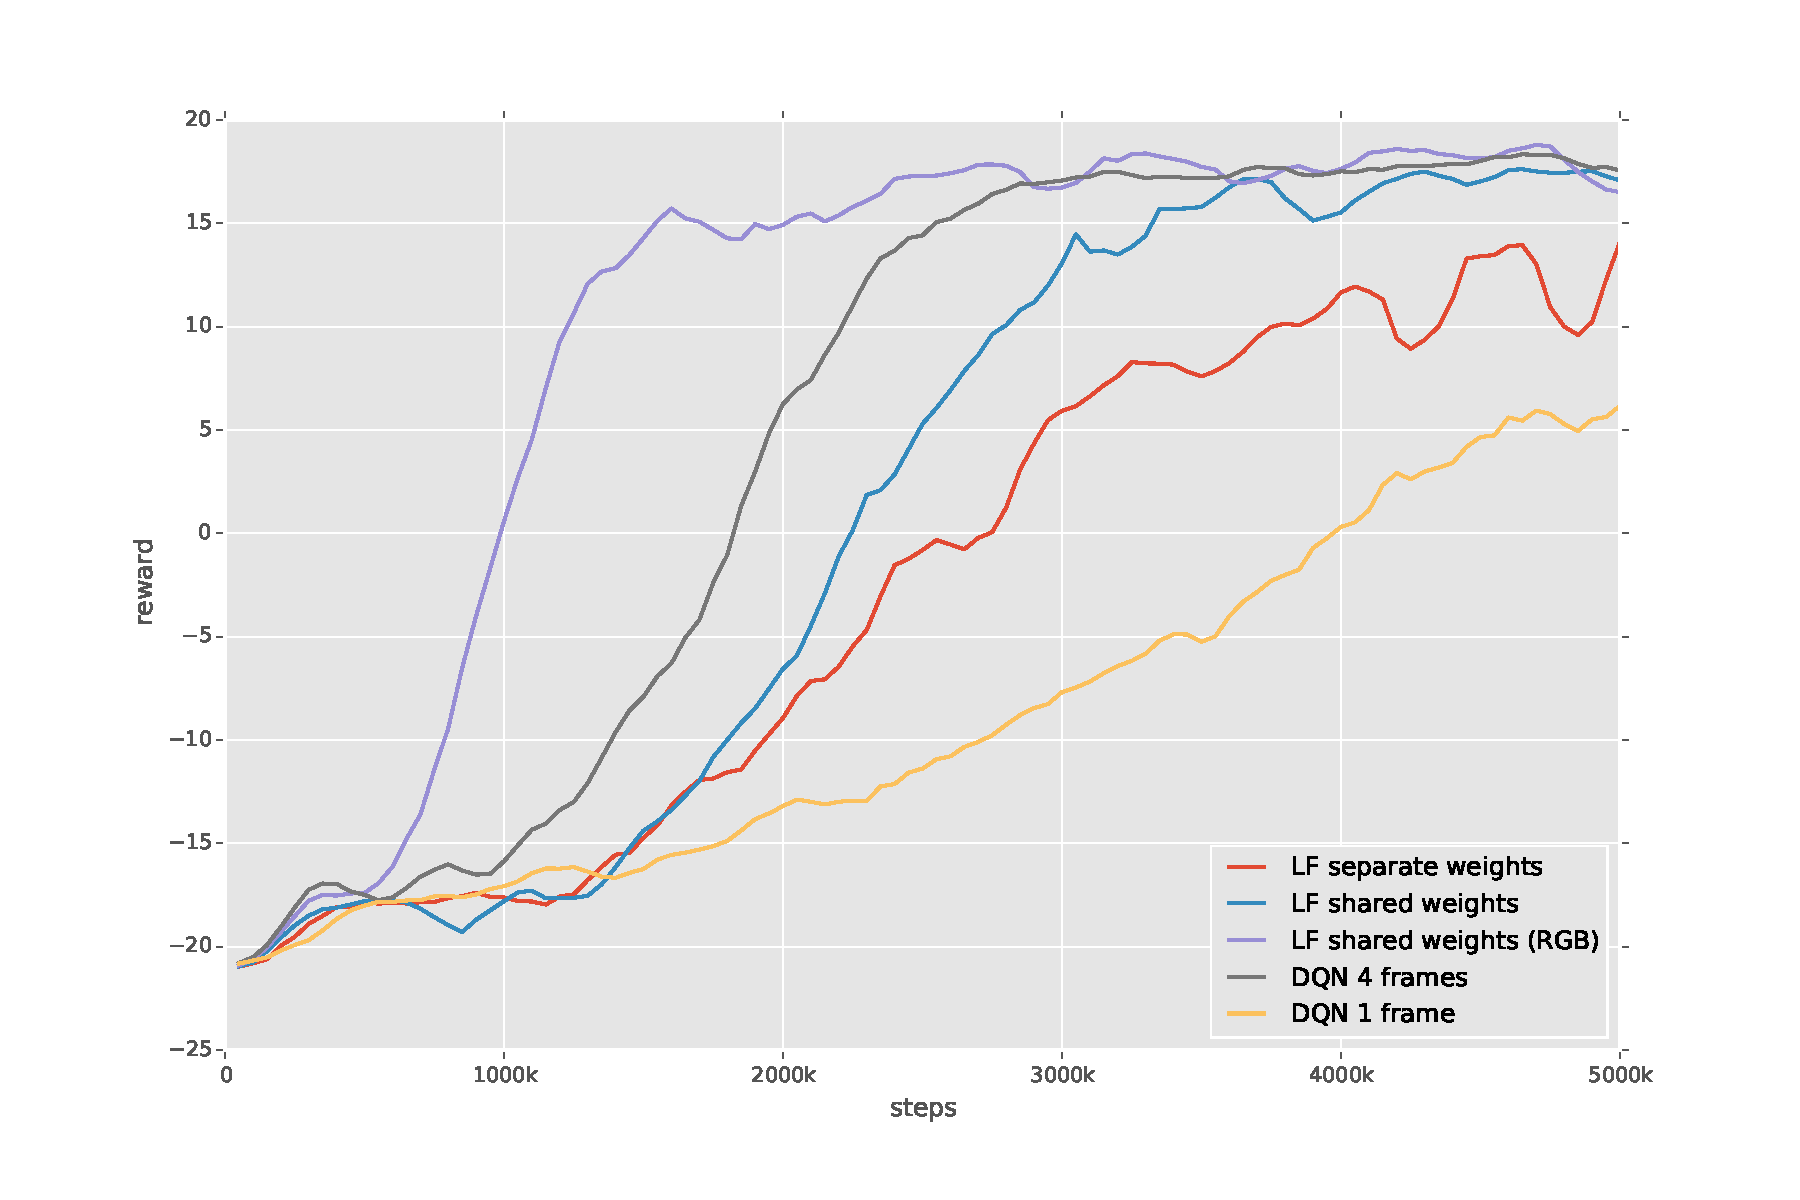
\includegraphics[width=1\linewidth]{late_fusion_pong_rewards.pdf}
  % TODO caption
  \caption{TODO}
  \label{fig:late_fusion_pong_rewards}
\end{figure}

\paragraph{}
Keeping the weights the same between convolutional layers on the same level
seems to offer an advantage over separate weights.
What this effectively does
is force the convolutional layers to learn the same features
so the output of the top convolutional layers
has exactly the same semantics.
This way the fully-connected layer has access
to the difference between frames at different time steps.

When not sharing weights each convolutional layer
has to learn features independently which slows down learning
and does not guarantee the same features will be learned.
In fact, this approach does not even outperform
the single-frame DQN.

\paragraph{}
While  the shared weights network
still does not learn as quickly as regular DQN,
giving the network access to RGB values offers obvious gains
in terms of learning speed.
The motivation behind access to three separate color channels
is that it is easier to learn a function on three variables
than just a single one
that is trying to encompass the same information
% TODO peter
and where a small shift in value can be associated
with a different entity on the screen.
With multiple inputs (color channels)
the network gains more representational power.

Figure \ref{fig:nips_vs_nature_rewards}
illustrates how some games can benefit
from added network capacity.

\paragraph{}
We can conclude that using two separate time steps
as input to the network
that are represented by the same learned features
offers gains
% TODO finish


\section{3D Convolutional Network Approach}
\label{sec:3d_convolutional_network_approach}
Building on the idea that time is an extra spatial dimension
and should not be handled differently
from image width or height,
I investigate 3D convolutional layers next.
In the original DQN implementation
the time dimension gets flattened immediately
by the first convolutional layer
and is not present explicitly
in its output;
only the first convolutional layer
has explicit access to time
because the 2D convolutional layer implementation
extends along the entire depth of the input.
Intuitively this means that only low-level
features over time can be learned
whereas we can easily imagine
more abstract features
that relate to time.
This is where the 3D convolutional network comes in,
in order to allow us to specify step size and stride across time
in order to control how time is propagated through the entire network.

\paragraph{}
The original 2D convolution setup in DQN
is exactly the same as a 3D convolution
with 4 input frames and only a single image channel (grayscale),
where the filter over time spans across all 4 input frames,
as illustrated by Figure \ref{fig:conv2d_time}.

A 3D convolutional layer gains an extra dimension
which can be used for image depth, like colors.
It also allows us to specify the filter size and stride over time.
Figure \ref{fig:conv3d_time} for example
employs a time filter size of 2 and a stride of 1.
Since this comes down to combining every consecutive pair of frames,
the output of the convolutional layer has a time dimension
that is shrunk by 1 compared to the number of input frames.

\begin{figure}[!htpb]
  \begin{subfigure}[t]{.45\textwidth}
    \centering
    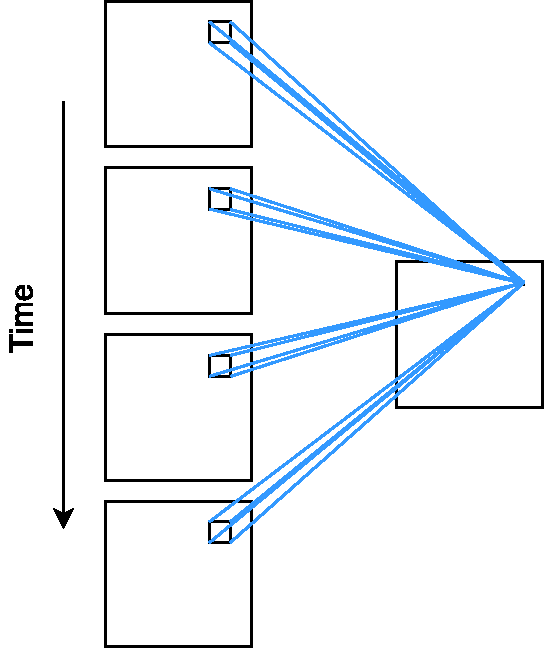
\includegraphics[width=.8\textwidth]{conv2d_time.pdf}
    \caption{
      2D convolution for a single feature as used by \cite{Mnih2013}.
      Since time is treated as image depth,
      a feature always spans across all time frames.
    }
    \label{fig:conv2d_time}
  \end{subfigure}
  \hfill
  \begin{subfigure}[t]{.45\textwidth}
    \centering
    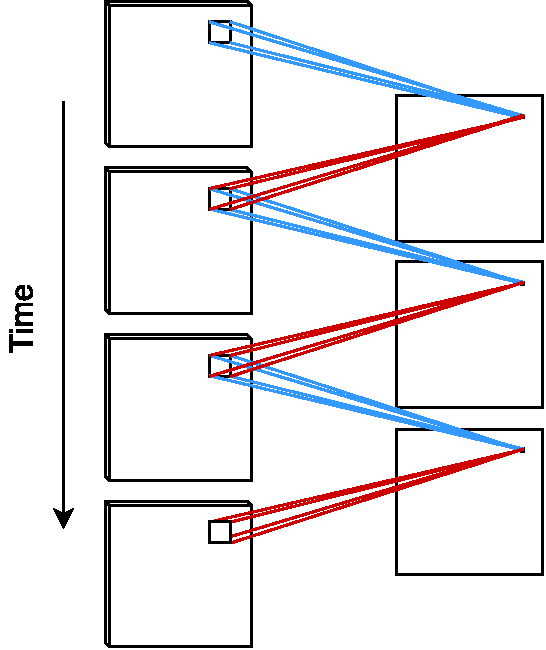
\includegraphics[width=.8\textwidth]{conv3d_time.pdf}
    % \vspace{.1\baselineskip}
    \caption{
      3D convolution for a single feature
      (depth slice of the convolutional layer)
      with 4 input frames
      and a time filter size of 2.
      Connections of the same color depict shared weights.
    }
    \label{fig:conv3d_time}
  \end{subfigure}
  \caption{
    Convolutions over time.
  }
  \label{fig:conv3d}
\end{figure}

\paragraph{}
The 3D Convolutional DQN
is again based entirely on the original DQN implementation
\parencite{Mnih2013},
with parameters in table \ref{tab:base}.

An example instantiation of the 3D convolutional DQN
can be found in Figure \ref{fig:conv3d_network}.
It leaves the amount if input channels unspecified;
in our case this can either be 1 for grayscale
or 3 for RGB values.
There are again two convolutional layers.
Since these make use of 3D convolutions,
filters over time can be specified.
Both layers in Figure \ref{fig:conv3d_network}
use a time filter size of 2,
so the time dimensions shrinks by 1 after each.
The fully-connected layer
still has a time dimension of size 2 to cope with in this example,
as opposed to a flattened time dimension in the original DQN architecture.

\begin{figure}[htpb]
  \centering
  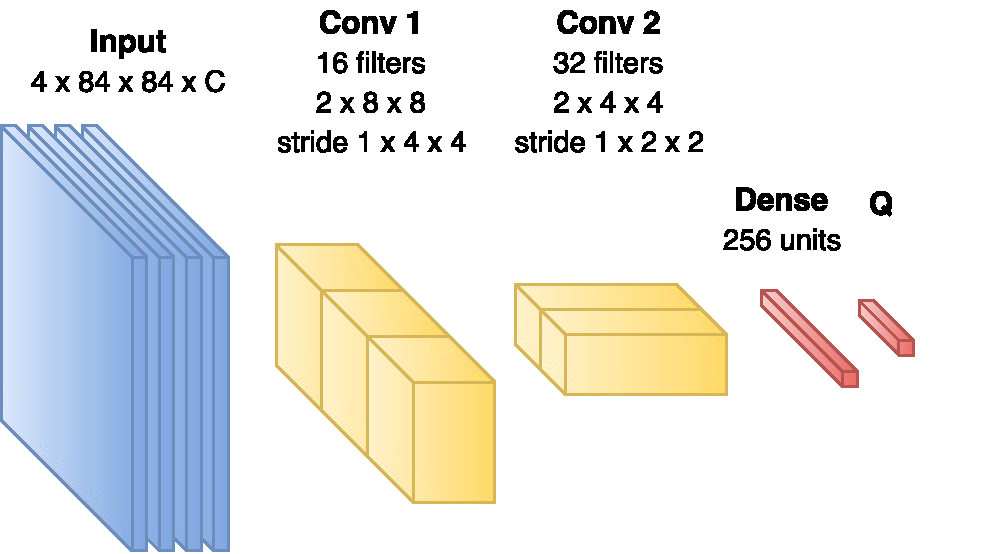
\includegraphics[width=\textwidth]{conv3d_network.pdf}
  % \vspace{.1\baselineskip}
  \caption{
    3D convolutional DQN.
    The input consists of 4 frames
    that can each have $C$ image channels.
    Both convolutional layers employ a time filter size of 2,
    meaning a single weight corresponds to
    two frames of the layer's input.
    Combined with a time stride of 1,
    the time dimension of the output of each consecutive layer
    is 1 smaller than its input.
  }
  \label{fig:conv3d_network}
\end{figure}

\subsection{Tuning}
\label{sub:conv3d_tuning}
There are different ways to combine time frames throughout the network.
A decision can be made between `merging'
(feeding multiple frames into a layer at a time)
early or later on.
For readability,
a network with time filter sizes
$n1$ and $n2$ for its two convolutional layers respectively
is denoted as a $(n1, n2)$ 3D convolutional network.

Next to varying time filter sizes
I also attempt a variation with an extra max pooling layer
right after the second convolutional layer
with a filter size of 2 across all dimensions.

Just like with the late fusion architecture
a variation that uses RGB image channels has also been attempted.

The learning curves for all of these networks
is shown in Figure \ref{conv3d_both}.

\begin{figure}[htpb]
  \centering
  \captionof{figure}{
    3D convolutional architecture comparison
  }
  \begin{subfigure}[t]{.49\linewidth}
    \caption{Reward learning curve}
    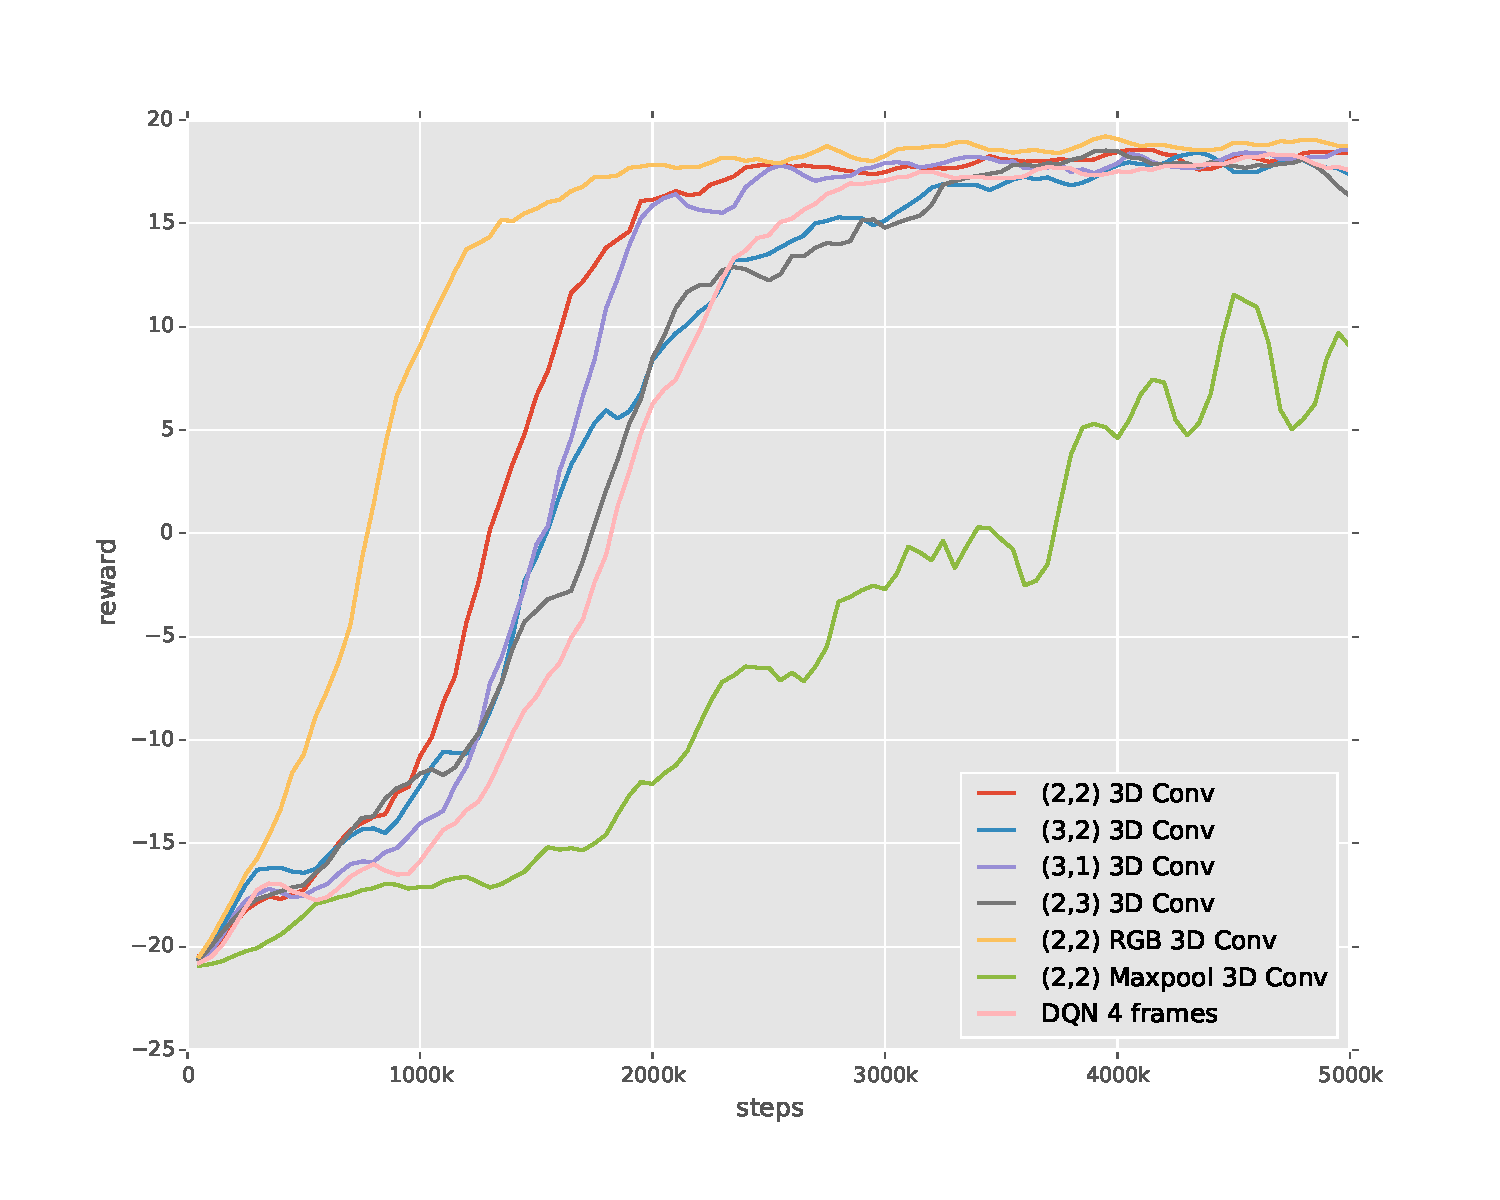
\includegraphics[width=1\textwidth]{conv3d_rewards}
  \end{subfigure}
  \begin{subfigure}[t]{.49\linewidth}
    \caption{Average Q learning curve}
    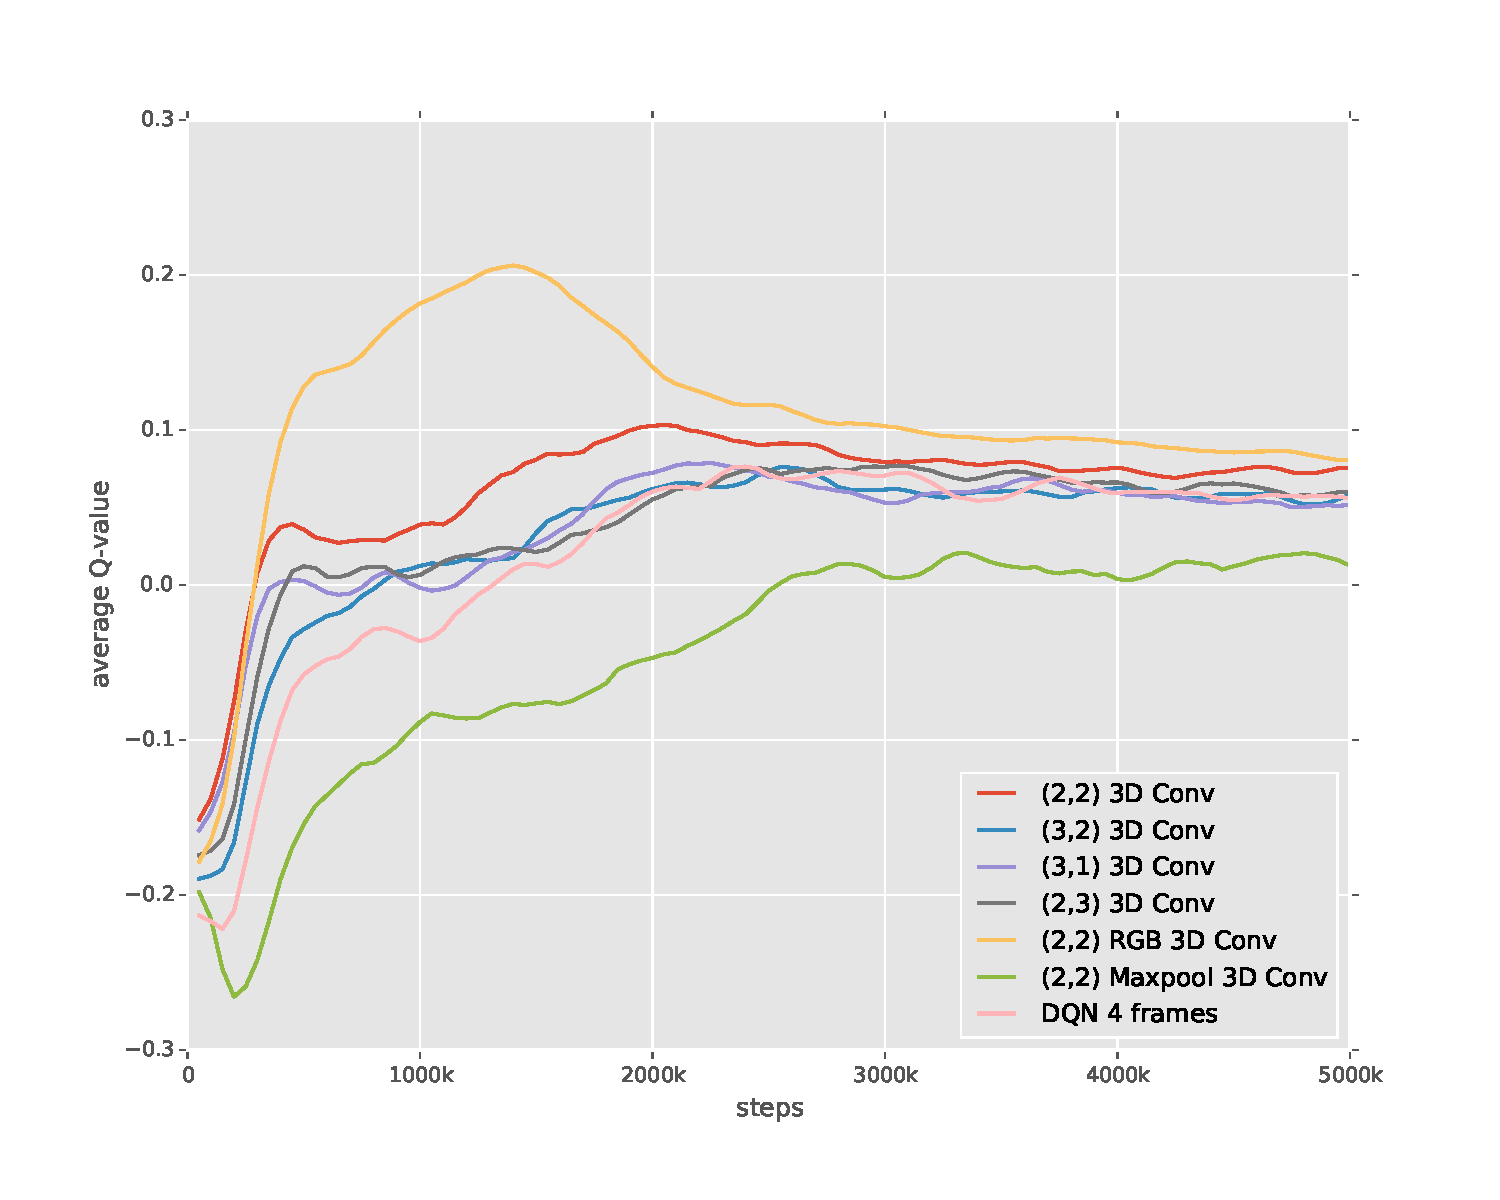
\includegraphics[width=1\textwidth]{conv3d_qs}
  \end{subfigure}
  \label{fig:conv3d_both}
\end{figure}

\paragraph{}
It can easily be seen that the max pooling variant
performs worst.
This is the one that supplies the least information
to the fully-connected layer.
Among the networks with different time filter sizes,
the $(2,2)$ variant performs best
yet it still does not outperform
the standard DQN architecture that uses 4 stacked frames.

Just as in the late fusion scenario,
using RGB-colored input performs noticeably better
and even fares better than standard DQN.

% TODO conclusion plis

\subsubsection{Flickering Pong}
While the 3D convolutional approach
did not do great compared to the regular DQN
on the basic scenario,
it is interesting to compare them
on a partially observable MDP
such as Flickering Pong.

For this purpose I used the $(2,2)$ 3D convolutional network from above
with greyscale input.
I then compared it against DQN by running both
networks first with 4 frames, then 10.
The results are illustrated in Figure \ref{fig:conv3d_flicker_both}.

\begin{figure}[htpb]
  \centering
  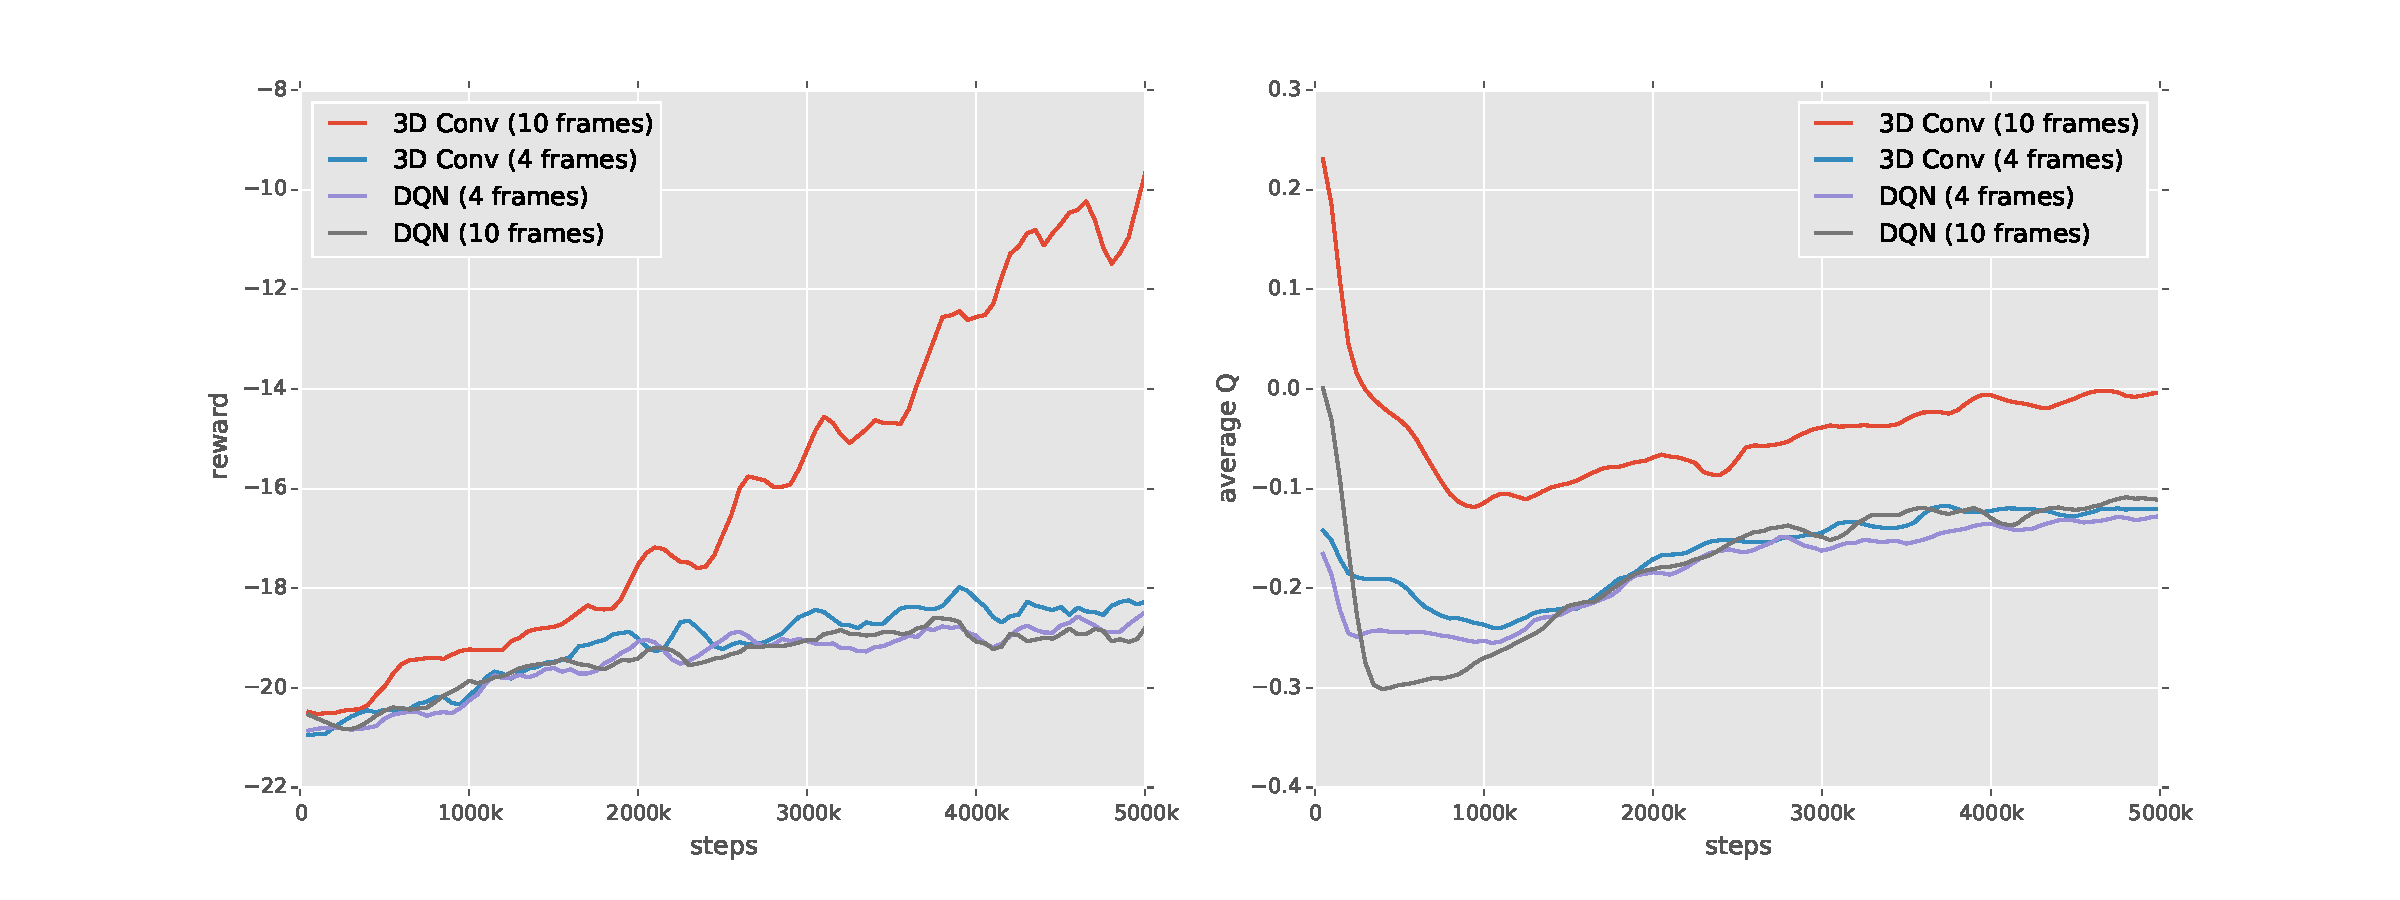
\includegraphics[width=1.0\linewidth]{conv3d_flicker_both.pdf}
  \caption{
    A comparison
    of reward and average Q-values over time
    of the 3D convolutional network versus DQN
    for the Flickering Pong game with $p=0.5$.
  }
  \label{fig:conv3d_flicker_both}
\end{figure}

\paragraph{}
While the 3D convolutional approach with 4 frames did not perform noticeably
better than DQN,
it did not perform worse either
which is definitely interesting considering
that it was outperformed on the regular Pong game.
Also interesting is that DQN does not seem to do any better when given more frames.

\paragraph{}
The surprising result is that the 3D convolutional network given 10 frames
did spectactulary better than any other approach in this comparison.
% TODO revise when more results for conv3d flicker
From the Q-value learning curve it can not be excluded that it is
even still learning while the other approaches seem to stagnate quickly
and the reward curve still shows an upward tendency.
The fact that the network requires more than 4 frames as input
to exhibit this behavior is not all that surprising altogether,
given that there is even a $6.25\%$ chance
that the input consists entirely of obscured frames.

\paragraph{}
% TODO peter peek
To conclude,
the 3D convolutional does not always outperform standard DQN
but can fare remarkably better
on the game Flickering Pong,
a true POMDP with stochastically obscured observations.



\section{Long Short-Term Memory Approach}
\label{sec:long_short_term_memory_approach}
The last approach I consider involves
the use of Long Short-Term Memory,
a specific kind of recurrent neural network
% TODO consider citation
that is capable of learning time dependencies
over arbitrary and unknown amounts of time.

The very same architecture I will discuss here
has been attempted by
\citeauthor{Hausknecht2015} (\citeyear{Hausknecht2015})
who found favorable results for some few games.
\citeauthor{Hausknecht2015}
concluded that few significant differences
were found with the original DQN architecture
and that no general benefit could be gained compared
to simply stacking frames.
One could however argue
that merely getting rid of the fixed window
which stacking automatically implies
presents a merit in its own right
and allows for better generalization of the architecture
to other problem domains.

\paragraph{}
Recall that the LSTM unit as we consider it here
contains three \textit{gates}
and an internal cell state (Section \ref{sec:lstm}).
The input gate and forget gate together govern
the content of the internal state,
which forms the memorizing core of the unit,
whereas the output gate
learns how to output the internal state
in order to create the gate's output.

\paragraph{}
The intuitive idea behind the use of LSTMs
is that the units will learn to remember important events
and then use that information at some later time
when it is required.
Given their goal,
they are especially useful in Partially Observable Markov Decision Processes
such as we have when considering only one Atari frame at a time.
Sadly, Atari games generally only have very short time dependencies
which make them an imperfect testbed for
long-term dependency learning
so we will focus on learning those instead.

\begin{figure}[htpb]
  \centering
  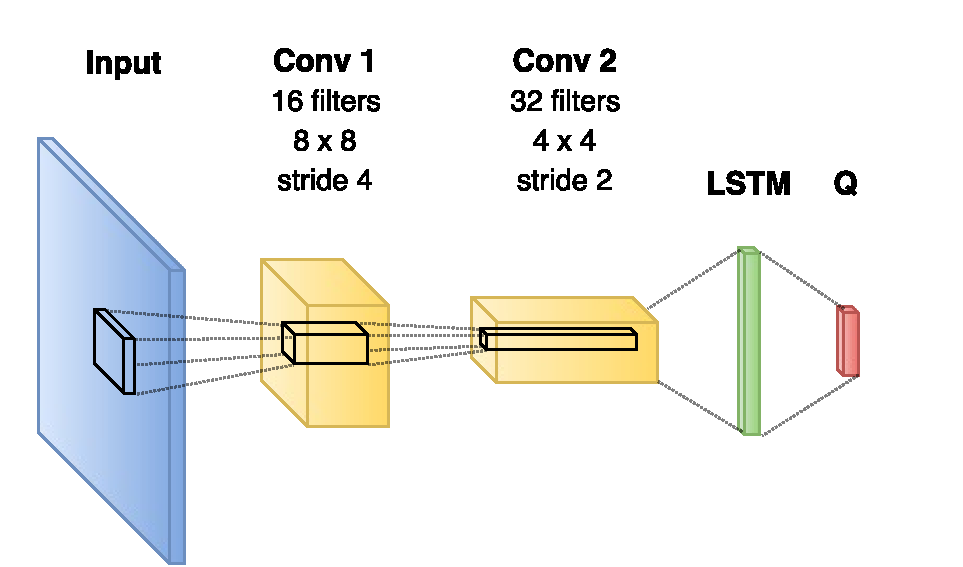
\includegraphics[width=.85\linewidth]{lstm_network.pdf}
  % TODO peter should I call this DQRN
  \caption{LSTM DQN}
  \label{fig:lstm_network}
\end{figure}

\subsection{Design and Training}
\label{sub:lstm_design_and_training}
The Long Short-Term Memory variant
of the deep Q-network
- or Deep Recurrent Q-Network,
as named by \ref{Hausknecht2015} -
is once again based on the DQN version
by \ref{Mnih2013},
with common parameters in Table \ref{tab:base}.

\paragraph{}
The network is constructed by taking out
the first fully-connected layer
and replacing it with an LSTM layer
with the same or different amount of units.
Everything else except the input stays the same.
Instead of stacking frames along the depth dimension of the input,
only one frame at a time now gets fed to the network.
It is up the LSTM layer to handle memorization across time.
Just like with the previous two approaches,
ridding ourselves of the stacked frames opens up the input depth dimension
once again
to be used for image channels like RGB values.

The network architecture is displayed in Figure \ref{fig:lstm_network}.

\paragraph{}
In the original Deep Q-Learning algorithm,
after each action selection
a mini-batch learning update would occur.
LSTMs require input frames to be observed in chronological order, however.
This learning approach would not work
because data gathering steps would be interleaved with mini-batch updates,
breaking the required flow of time,
so the LSTM units
would consider the mini-batch to follow the observed frame right before the update
which is of course not the case.
On top of that, mini-batches contain random samples
in order to break correlation
between consecutive frames
while LSTMs, again, require uninterrupted sequences.

\paragraph{}
In order to accomodate the new requirements,
I adapted the Deep Q-Learning algorithm
to keep sequential information intact at all times.
First off,
this required a new sampling method.
Instead of sampling 32 random samples,
I now sample \textit{random sequences}.
This is done by selecting a single random time step,
then including consecutive time steps
until either the batch size (by default 32)
is reached or the episode terminates.
This batch then gets treated like it would be normally,
feeding it into the learning update while keeping the order intact
so the LSTM's internal state could follow along.

\paragraph{}
This brings me to the internal state reset and backup.
At the start of any episode,
the LSTM's internal state along with its output history
gets reset to initial values.
These initial values can be fixed and supplied
by the network designer
or even learned dynamically.
The reset is required to make clear to the LSTM
that the first state of an episode
does not follow the terminal state of the last episode.

A parameter \textit{backup} and subsequent reset
on the other hand
occur at the start of every mini-batch learning update.
This is done so the sequential mini-batch
forms an isolated sequence of events
and no accidental information from before the update gets carried into the update
by the LSTM's internal memory.
After the update
the internal state and output history
are restored from the backup
so the agent can go on gathering data
as if no interruption had just occurred.

\subsection{Tuning}
\label{sub:lstm_tuning}



\section{Conclusions}
\label{sec:conclusions}


